From the given information,
\begin{align}
\vec{m}_1 = \myvec{-3\\ 2k\\ 2},\,  \vec{m}_2 =\myvec{3k\\ 1\\ -5} 
\\
	\implies \myvec{-3& 2k& 2}^{\top} \myvec{3k\\ 1\\ -5} =0
	\\
	\implies k = -\frac{10}{7}
\end{align}
\iffalse
See 
     \figref{fig:chapters/12/11/4/6/1}
\begin{figure}[H]
  \centering
   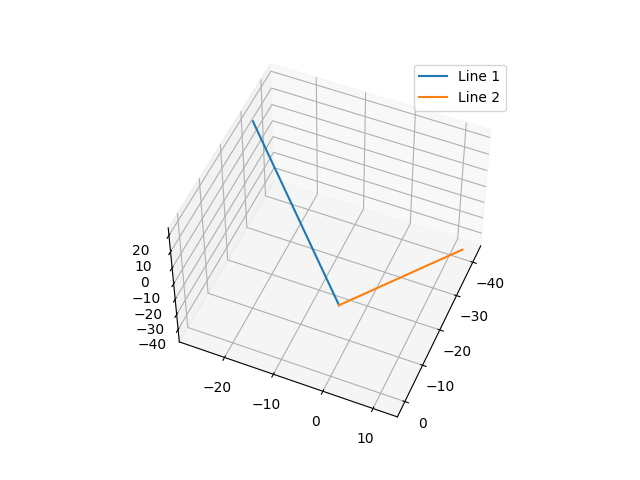
\includegraphics[width=0.75\columnwidth]{chapters/12/11/4/6/figs/line_1.png}
    \caption{lines represented for the given points and direction vector with k=$\frac{-10}{7}$}
     \label{fig:chapters/12/11/4/6/1}
     \end{figure}  
     \fi


